\section{Testing}\label{Testing}
    [The testing setup and suite. The testing method and how we did the testing.]
    
    %% To be written, about the testing routines and NS3 and the test results. 
    
    \subsection{About the testing suite}\label{Testing:About}
        \subsubsection{Test Client}\label{Testing:About:Client}
            In this section we will shortly describe the test client used for testing, \ref{attachment?}"EchoClientClient.jar".
            % TODO: fix ref.

            The client starts by reading its configuration file. Its filename can be provided as the only command line argument, otherwise it defaults to "client.config'. This configuration file contains variables such as username, password, role, service to contact, what the request should be, how many requests to send and with what interval it should send them at, and some describing what to log.

            The client expects the request to contain '{REQID}' as part of the request message, and before sending it, the client will replace it with '{REQID=XX}' where 'XX' is the number of the request. This way the client can check that it gets the right response by checking whether '{REQID=XX}' is present in the response, and whether the ID is correct. This makes validating the response from the service easier, but it restricts the service to put the request message somewhere in the response. Another side effect of this being the only validation is that other errors in the response are not easily detected as long as the '{REQID=XX}' is there. If for example the response is cut short, by the stream being cut, as long as the ID is present it will be treated as valid. The client also prints the length of the response, so scripts that parse the results can pick up on responses with abnormal lengths.

            After reading the configuration file the client makes an instance of the client library\ref{some client library reference} 
            % TODO: fix ref.
            using the username, password and role, and itself as an ExceptionHandler. By implementing itself as the ExceptionHandler the client will be notified about all the exceptions ocurring in the client library, the client does not act upon these exceptions, but it does log them. A normal client might want to send a request again here.
            
            A timer is used to start the sending/receiving in a new thread at the interval specified and the number of times specified. Starting new threads for every request and sending at a small interval is a good way to test how the client library handles concurrent requests.

            The actual sending and receiving of data is rather simple, as you can see in this code snippet:
            \begin{figure}[h]
                \centering
                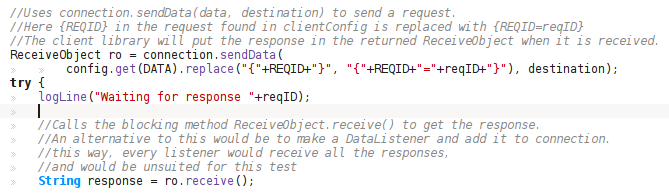
\includegraphics[width=\textwidth]{TestClientSending}
                \caption{Sending and Receiving in the Test Client}
                This code snippet shows how sending and receiving is done in the test client using the client library.
                \label{fig:TestClientSending}
            \end{figure}
            \\
            For more details about configuring the test client read the example configuration provided \ref{attachments:client.config}. For more detailed information on how the test client works, the java file with javadoc is provided \ref{attachments:TestClient.java}.
            % TODO: fix refs.

        \subsubsection{Test Service}\label{Testing:About:Service}
            In this section we will shortly describe the test service used for testing, \ref{attachment?}"EchoServiceLargeReply.war".
            % TODO: fix ref.

            The test service is very simple and deployable with GlassFish. It expects a request like this:
            \begin{figure}[h]
                \centering
                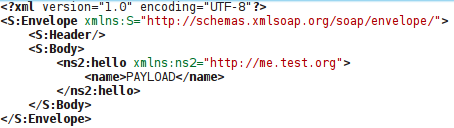
\includegraphics[width=\textwidth]{TestServiceRequest}
                \label{fig:TestServiceRequest}
            \end{figure}
            \\
            And responds like this:
            \begin{figure}[h]
                \centering
                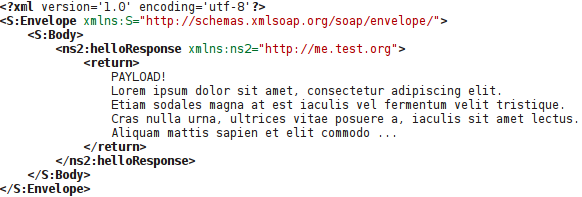
\includegraphics[width=\textwidth]{TestServiceResponse}
                \label{fig:TestServiceResponse}
            \end{figure}
            With PAYLOAD intact, and 10Kb of Lorem Ipsum\footnote{\URL{http://www.lipsum.com/} - simply dummy text}. We add these 10Kb's of text to ensure that the response is considerably larger than the request, which should get us more realistic results when testing. We also sends the original payload back so the test client can easily identify which request was responded to.
            
    % mobiemu (NS3) 
    % test cases.
    % test results.
    % test setup
